\documentclass{standalone}
\usepackage{tikz}
\usetikzlibrary{patterns, positioning}

\begin{document}
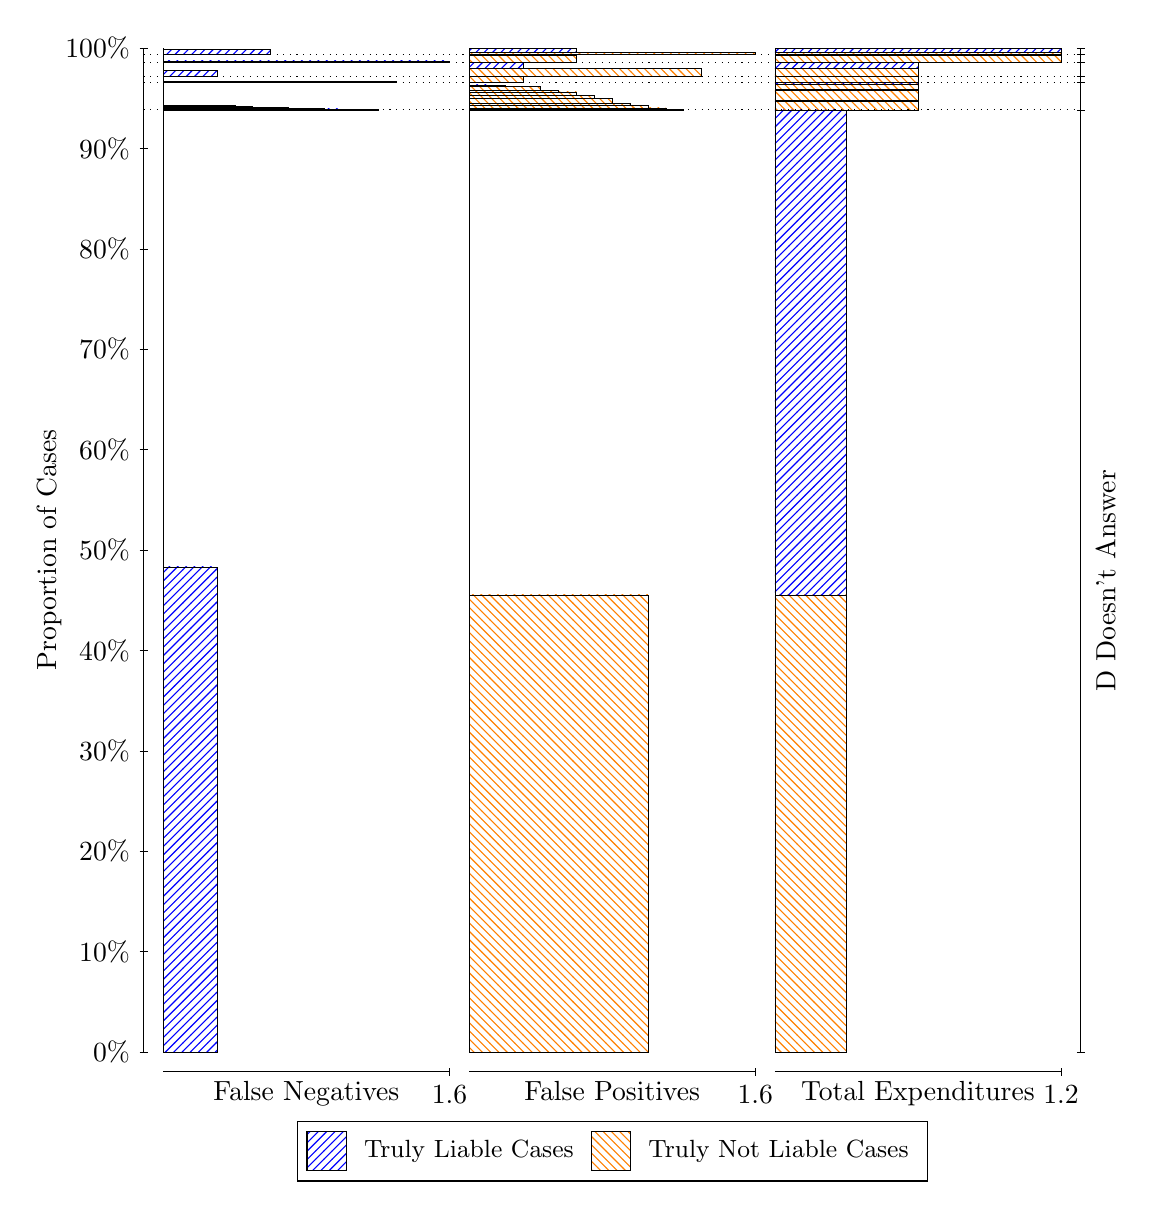
\begin{tikzpicture}
\draw[black, very thin] (1.5,1.75) -- (1.5,14.5);
\node[rotate=90, anchor=center] at (0.3, 8.125) {Proportion of Cases};
\draw[black, very thin] (1.45,1.75) -- (1.55,1.75);
\node[anchor=east] at (1.45, 1.75) {0\%};
\draw[black, very thin] (1.45,3.025) -- (1.55,3.025);
\node[anchor=east] at (1.45, 3.025) {10\%};
\draw[black, very thin] (1.45,4.3) -- (1.55,4.3);
\node[anchor=east] at (1.45, 4.3) {20\%};
\draw[black, very thin] (1.45,5.575) -- (1.55,5.575);
\node[anchor=east] at (1.45, 5.575) {30\%};
\draw[black, very thin] (1.45,6.85) -- (1.55,6.85);
\node[anchor=east] at (1.45, 6.85) {40\%};
\draw[black, very thin] (1.45,8.125) -- (1.55,8.125);
\node[anchor=east] at (1.45, 8.125) {50\%};
\draw[black, very thin] (1.45,9.4) -- (1.55,9.4);
\node[anchor=east] at (1.45, 9.4) {60\%};
\draw[black, very thin] (1.45,10.675) -- (1.55,10.675);
\node[anchor=east] at (1.45, 10.675) {70\%};
\draw[black, very thin] (1.45,11.95) -- (1.55,11.95);
\node[anchor=east] at (1.45, 11.95) {80\%};
\draw[black, very thin] (1.45,13.225) -- (1.55,13.225);
\node[anchor=east] at (1.45, 13.225) {90\%};
\draw[black, very thin] (1.45,14.5) -- (1.55,14.5);
\node[anchor=east] at (1.45, 14.5) {100\%};

\draw[black, very thin] (13.4,1.75) -- (13.4,14.5);
\draw[black, very thin] (13.35,1.75) -- (13.45,1.75);
\node[anchor=west] at (13.35, 1.75) {};
\draw[black, very thin] (13.35,13.715) -- (13.45,13.715);
\node[anchor=west] at (13.35, 13.715) {};
\draw[black, very thin] (13.35,14.066) -- (13.45,14.066);
\node[anchor=west] at (13.35, 14.066) {};
\draw[black, very thin] (13.35,14.141) -- (13.45,14.141);
\node[anchor=west] at (13.35, 14.141) {};
\draw[black, very thin] (13.35,14.318) -- (13.45,14.318);
\node[anchor=west] at (13.35, 14.318) {};
\draw[black, very thin] (13.35,14.423) -- (13.45,14.423);
\node[anchor=west] at (13.35, 14.423) {};
\draw[black, very thin] (13.35,14.5) -- (13.45,14.5);
\node[anchor=west] at (13.35, 14.5) {};

\draw[black, very thin, pattern color=blue, pattern=north east lines] (1.75,1.75) rectangle (2.4312,7.9097);
\draw[black, very thin, pattern color=orange, pattern=north west lines] (1.75,7.9097) rectangle (1.75,13.715);
\draw[black, very thin, pattern color=blue, pattern=north east lines] (1.75,13.715) rectangle (4.475,13.721);
\draw[black, very thin, pattern color=blue, pattern=north east lines] (1.75,13.721) rectangle (4.2479,13.722);
\draw[black, very thin, pattern color=blue, pattern=north east lines] (1.75,13.722) rectangle (4.0208,13.727);
\draw[black, very thin, pattern color=blue, pattern=north east lines] (1.75,13.727) rectangle (3.7937,13.729);
\draw[black, very thin, pattern color=blue, pattern=north east lines] (1.75,13.729) rectangle (3.7937,13.732);
\draw[black, very thin, pattern color=blue, pattern=north east lines] (1.75,13.732) rectangle (3.5667,13.738);
\draw[black, very thin, pattern color=blue, pattern=north east lines] (1.75,13.738) rectangle (3.3396,13.742);
\draw[black, very thin, pattern color=blue, pattern=north east lines] (1.75,13.742) rectangle (3.1125,13.75);
\draw[black, very thin, pattern color=blue, pattern=north east lines] (1.75,13.75) rectangle (2.8854,13.757);
\draw[black, very thin, pattern color=blue, pattern=north east lines] (1.75,13.757) rectangle (2.6583,13.771);
\draw[black, very thin, pattern color=orange, pattern=north west lines] (1.75,13.771) rectangle (1.75,14.066);
\draw[black, very thin, pattern color=blue, pattern=north east lines] (1.75,14.066) rectangle (4.7021,14.072);
\draw[black, very thin, pattern color=orange, pattern=north west lines] (1.75,14.072) rectangle (1.75,14.141);
\draw[black, very thin, pattern color=blue, pattern=north east lines] (1.75,14.141) rectangle (2.4312,14.215);
\draw[black, very thin, pattern color=orange, pattern=north west lines] (1.75,14.215) rectangle (1.75,14.318);
\draw[black, very thin, pattern color=blue, pattern=north east lines] (1.75,14.318) rectangle (5.3833,14.337);
\draw[black, very thin, pattern color=orange, pattern=north west lines] (1.75,14.337) rectangle (1.75,14.423);
\draw[black, very thin, pattern color=blue, pattern=north east lines] (1.75,14.423) rectangle (3.1125,14.482);
\draw[black, very thin, pattern color=orange, pattern=north west lines] (1.75,14.482) rectangle (1.75,14.5);
\draw[black, very thin, pattern color=orange, pattern=north west lines] (5.6333,1.75) rectangle (7.9042,7.5557);
\draw[black, very thin, pattern color=blue, pattern=north east lines] (5.6333,7.5557) rectangle (5.6333,13.715);
\draw[black, very thin, pattern color=orange, pattern=north west lines] (5.6333,13.715) rectangle (8.3583,13.722);
\draw[black, very thin, pattern color=orange, pattern=north west lines] (5.6333,13.722) rectangle (8.1313,13.739);
\draw[black, very thin, pattern color=orange, pattern=north west lines] (5.6333,13.739) rectangle (7.9042,13.769);
\draw[black, very thin, pattern color=orange, pattern=north west lines] (5.6333,13.769) rectangle (7.6771,13.801);
\draw[black, very thin, pattern color=orange, pattern=north west lines] (5.6333,13.801) rectangle (7.45,13.856);
\draw[black, very thin, pattern color=orange, pattern=north west lines] (5.6333,13.856) rectangle (7.2229,13.901);
\draw[black, very thin, pattern color=orange, pattern=north west lines] (5.6333,13.901) rectangle (6.9958,13.944);
\draw[black, very thin, pattern color=orange, pattern=north west lines] (5.6333,13.944) rectangle (6.7687,13.959);
\draw[black, very thin, pattern color=orange, pattern=north west lines] (5.6333,13.959) rectangle (6.5417,14.01);
\draw[black, very thin, pattern color=blue, pattern=north east lines] (5.6333,14.01) rectangle (6.0875,14.025);
\draw[black, very thin, pattern color=blue, pattern=north east lines] (5.6333,14.025) rectangle (5.8604,14.031);
\draw[black, very thin, pattern color=blue, pattern=north east lines] (5.6333,14.031) rectangle (5.6333,14.066);
\draw[black, very thin, pattern color=orange, pattern=north west lines] (5.6333,14.066) rectangle (6.3146,14.135);
\draw[black, very thin, pattern color=blue, pattern=north east lines] (5.6333,14.135) rectangle (5.6333,14.141);
\draw[black, very thin, pattern color=orange, pattern=north west lines] (5.6333,14.141) rectangle (8.5854,14.244);
\draw[black, very thin, pattern color=blue, pattern=north east lines] (5.6333,14.244) rectangle (6.3146,14.318);
\draw[black, very thin, pattern color=orange, pattern=north west lines] (5.6333,14.318) rectangle (6.9958,14.403);
\draw[black, very thin, pattern color=blue, pattern=north east lines] (5.6333,14.403) rectangle (5.6333,14.423);
\draw[black, very thin, pattern color=orange, pattern=north west lines] (5.6333,14.423) rectangle (9.2667,14.441);
\draw[black, very thin, pattern color=blue, pattern=north east lines] (5.6333,14.441) rectangle (6.9958,14.5);
\draw[black, very thin, pattern color=orange, pattern=north west lines] (9.5167,1.75) rectangle (10.425,7.5557);
\draw[black, very thin, pattern color=blue, pattern=north east lines] (9.5167,7.5557) rectangle (10.425,13.715);
\draw[black, very thin, pattern color=orange, pattern=north west lines] (9.5167,13.715) rectangle (11.333,13.818);
\draw[black, very thin, pattern color=blue, pattern=north east lines] (9.5167,13.818) rectangle (11.333,13.839);
\draw[black, very thin, pattern color=orange, pattern=north west lines] (9.5167,13.839) rectangle (11.333,13.963);
\draw[black, very thin, pattern color=blue, pattern=north east lines] (9.5167,13.963) rectangle (11.333,13.976);
\draw[black, very thin, pattern color=orange, pattern=north west lines] (9.5167,13.976) rectangle (11.333,14.044);
\draw[black, very thin, pattern color=blue, pattern=north east lines] (9.5167,14.044) rectangle (11.333,14.066);
\draw[black, very thin, pattern color=orange, pattern=north west lines] (9.5167,14.066) rectangle (11.333,14.135);
\draw[black, very thin, pattern color=blue, pattern=north east lines] (9.5167,14.135) rectangle (11.333,14.141);
\draw[black, very thin, pattern color=orange, pattern=north west lines] (9.5167,14.141) rectangle (11.333,14.244);
\draw[black, very thin, pattern color=blue, pattern=north east lines] (9.5167,14.244) rectangle (11.333,14.318);
\draw[black, very thin, pattern color=orange, pattern=north west lines] (9.5167,14.318) rectangle (13.15,14.403);
\draw[black, very thin, pattern color=blue, pattern=north east lines] (9.5167,14.403) rectangle (13.15,14.423);
\draw[black, very thin, pattern color=orange, pattern=north west lines] (9.5167,14.423) rectangle (13.15,14.441);
\draw[black, very thin, pattern color=blue, pattern=north east lines] (9.5167,14.441) rectangle (13.15,14.5);
\draw[black, dotted] (1.5,13.715) -- (13.4,13.715);
\draw[black, dotted] (1.5,14.066) -- (13.4,14.066);
\draw[black, dotted] (1.5,14.141) -- (13.4,14.141);
\draw[black, dotted] (1.5,14.318) -- (13.4,14.318);
\draw[black, dotted] (1.5,14.423) -- (13.4,14.423);
\draw[black, very thin] (1.75,1.5) -- (5.3833,1.5);
\node[anchor=north] at (3.5667, 1.5) {False Negatives};
\draw[black, very thin] (5.3833,1.45) -- (5.3833,1.55);
\node[anchor=north] at (5.3833, 1.45) {1.6};

\draw[black, very thin] (5.6333,1.5) -- (9.2667,1.5);
\node[anchor=north] at (7.45, 1.5) {False Positives};
\draw[black, very thin] (9.2667,1.45) -- (9.2667,1.55);
\node[anchor=north] at (9.2667, 1.45) {1.6};

\draw[black, very thin] (9.5167,1.5) -- (13.15,1.5);
\node[anchor=north] at (11.333, 1.5) {Total Expenditures};
\draw[black, very thin] (13.15,1.45) -- (13.15,1.55);
\node[anchor=north] at (13.15, 1.45) {1.2};

\node[black, centered, rotate=90] at (13.72, 7.7327) {D Doesn't Answer};






\draw (7.449999999999999,1.5) node[draw=none] (baseCoordinate) {};
\begin{scope}[align=center]
        \matrix[scale=0.5, draw=black, below=0.5cm of baseCoordinate, nodes={draw}, column sep=0.1cm]{
            \node[rectangle, draw, minimum width=0.5cm, minimum height=0.5cm, pattern=north east lines, pattern color=blue] {}; &
            \node[draw=none, font=\small] (B) {Truly Liable Cases}; &
            \node[rectangle, draw, minimum width=0.5cm, minimum height=0.5cm, pattern=north west lines, pattern color=orange] {}; &
            \node[draw=none, font=\small] (B) {Truly Not Liable Cases}; \\
            };
\end{scope}

\end{tikzpicture}
\end{document}